\change{\subsection{Уравнение Кеплера}}

\begin{wrapfigure}[15]{r}{0.48\tw}
	\centering
%	\vspace{-0.3pc}
	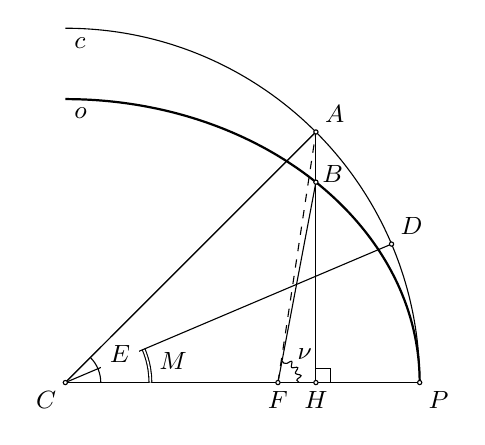
\begin{tikzpicture}[scale = 0.9]
	\small
	
	\draw (0, 5) arc(90:0:5);
	\draw[thick] (0, 4) arc(90:0:5 and 4);
	\draw (0, 0) -- (5, 0);
	
	\draw (0, 0) -- (3.536, 3.536); %%% Угол E = 45 градусов
	\draw (3, 0) -- (3.536, 2.828); %%% a * cos(45) * (b / a)
	\draw[dashed] (3, 0) -- (3.536, 3.536); %%% a * cos(45) * (b / a)
	
	
	\draw (0.5, 0) arc(0:45:0.5);
	\draw[double] (1.2, 0) arc(0:23:1.2);
	\draw[decoration={snake, segment length=1mm,
            amplitude=0.3mm}, decorate] (3.3, 0) arc(0:79.26:0.3);
	\draw (3.536, 3.536) -- (3.536, 0);
	
	\draw (0, 0) node [anchor=north east] {$C$};
	\draw (3, 0) node [anchor=north] {$F$};
	\draw (3.536, 3.536) node[anchor=south west] {$A$};
	\draw (3.5, 2.7) node[anchor=south west] {$B$};
	\draw (1.2, 0.05) node[anchor=south west] {$M$};
	\draw (0, 0) -- (4.603, 1.954); %%% a * cos(23)
	\draw (0.5, 0.15) node[anchor=south west, fill=white] {$E$};
	\draw (0, 0) -- (3.536, 3.536);
	\draw (3.15, 0.2) node[anchor=south west] {$\nu$};
	
	\draw (5, 0) node [anchor= north west] {$P$};
	\draw (3.536, 0) node [anchor= north] {$H$};
	\draw (4.603, 1.954) node [anchor=south west] {$D$};
	\draw (0, 5) node [anchor=north west] {$c$};
	\draw (0, 4) node [anchor=north west] {$o$};
	
	\draw[fill=white] (3.536, 3.536) circle (0.03); 	 %%% A
	\draw[fill=white] (3.536, 2.828) circle (0.03); 	 %%% B
	\draw[fill=white] (0, 0) circle (0.03);			 %%% C
	\draw[fill=white] (4.603, 1.954) circle (0.03); 	 %%% D
	\draw[fill=white] (3, 0) circle (0.03); 	         %%% F
	\draw[fill=white] (3.536, 0) circle (0.03);      %%% H
	\draw[fill=white] (5, 0) circle (0.03);          %%% P
	
	\draw (3.736, 0) -- (3.736, 0.2) -- (3.536, 0.2);

\end{tikzpicture}
	\captionof{figure}{К выводу уравнения Кеплера}
	\label{fig:kepler-eq}
\end{wrapfigure}\change{Рассмотрим эллиптическую орбиту $o$ с центром в точке $C$, центральным телом в фокусе $F$ и большой полуосью $a$. Обозначим за $P$ перицентр данной орбиты, тогда $|CP| = a$. Рассмотрим также окружность $c$, с центром в точке в точке $C$ и радиусом $a$, очевидно, эта окружность будет касаться эллипса внешним образом в точке~$P$. Выберем на эллипсе произвольную точку $B$. Проведем через нее прямую, параллельную малой оси эллипса. Точку пересечения полученной прямой с окружностью $c$ назовем $A$. Угол $E = \angle ACP$ называется \term{эксцентрической аномалией} точки $B$.
}

\change{Получим связь средней аномалии $M$ с эксцентрической~--- $E$. Прежде всего напомним, что эллипс является результатом действия аффинного преобразования сжатия (вдоль малой оси) на окружность с радиусом~$a$. И, наоборот, окружность под действием растяжения переходит в эллипс. В наших обозначениях будем считать, что окружность $o$ под действием сжатия $\xi$ с коэффициентом $a/b$ переходит в эллипс $o$. 
}

\begin{figure}[h!]
\begin{subfigure}{0.47\tw}
	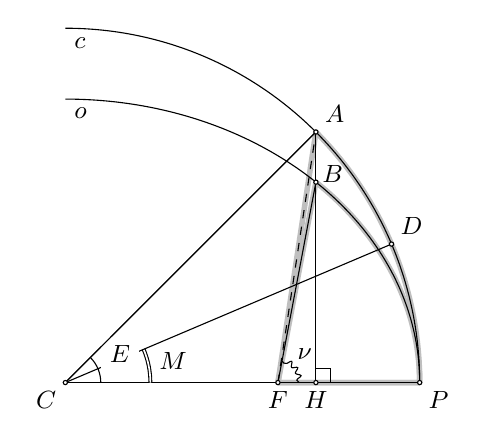
\begin{tikzpicture}[scale = 0.9]
	\small
	
	\draw[line width=2pt, lightgray, line join = round] (5, 0) arc(0:45:5) -- (3, 0) -- cycle;
	\draw[line width=2pt, lightgray, line join = round] (5, 0) arc(0:45:5 and 4) -- (3, 0) -- cycle;
	
	\draw (0, 5) arc(90:0:5);
	\draw (0, 4) arc(90:0:5 and 4);
	\draw (0, 0) -- (5, 0);
	
	\draw (0, 0) -- (3.536, 3.536); %%% Угол E = 45 градусов
	\draw (3, 0) -- (3.536, 2.828); %%% a * cos(45) * (b / a)
	\draw[dashed] (3, 0) -- (3.536, 3.536); %%% a * cos(45) * (b / a)
	
	
	\draw (0.5, 0) arc(0:45:0.5);
	\draw[double] (1.2, 0) arc(0:23:1.2);
	\draw[decoration={snake, segment length=1mm,
            amplitude=0.3mm}, decorate] (3.3, 0) arc(0:79.26:0.3);
	\draw (3.536, 3.536) -- (3.536, 0);
	
	\draw (0, 0) node [anchor=north east] {$C$};
	\draw (3, 0) node [anchor=north] {$F$};
	\draw (3.536, 3.536) node[anchor=south west] {$A$};
	\draw (3.5, 2.7) node[anchor=south west] {$B$};
	\draw (1.2, 0.05) node[anchor=south west] {$M$};
	\draw (0, 0) -- (4.603, 1.954); %%% a * cos(23)
	\draw (0.5, 0.15) node[anchor=south west, fill=white] {$E$};
	\draw (0, 0) -- (3.536, 3.536);
	\draw (3.15, 0.2) node[anchor=south west] {$\nu$};
	
	\draw (5, 0) node [anchor= north west] {$P$};
	\draw (3.536, 0) node [anchor= north] {$H$};
	\draw (4.603, 1.954) node [anchor=south west] {$D$};
	\draw (0, 5) node [anchor=north west] {$c$};
	\draw (0, 4) node [anchor=north west] {$o$};
	
	\draw[fill=white] (3.536, 3.536) circle (0.03); 	 %%% A
	\draw[fill=white] (3.536, 2.828) circle (0.03); 	 %%% B
	\draw[fill=white] (0, 0) circle (0.03);			 %%% C
	\draw[fill=white] (4.603, 1.954) circle (0.03); 	 %%% D
	\draw[fill=white] (3, 0) circle (0.03); 	         %%% F
	\draw[fill=white] (3.536, 0) circle (0.03);      %%% H
	\draw[fill=white] (5, 0) circle (0.03);          %%% P
	
	\draw (3.736, 0) -- (3.736, 0.2) -- (3.536, 0.2);

\end{tikzpicture}
\caption{Секторы $\sector BFP$ и $\sector AFP$}
\end{subfigure}
\hfill
\begin{subfigure}{0.47\tw}
	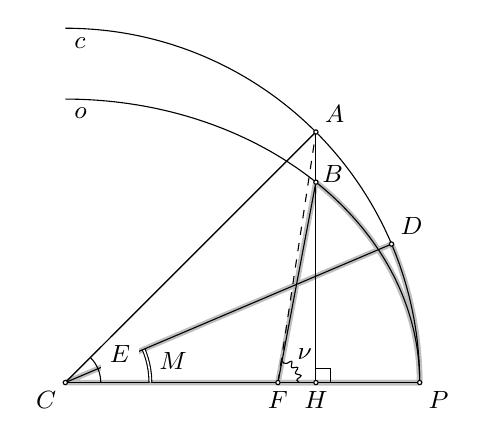
\begin{tikzpicture}[scale = 0.9]
	\small
	
	\draw[line width=2pt, lightgray, line join = round] (5, 0) arc(0:23:5) -- (0, 0) -- cycle;
	\draw[line width=2pt, lightgray, line join = round] (5, 0) arc(0:45:5 and 4) -- (3, 0) -- cycle;
	
	\draw (0, 5) arc(90:0:5);
	\draw (0, 4) arc(90:0:5 and 4);
	\draw (0, 0) -- (5, 0);
	
	\draw (0, 0) -- (3.536, 3.536); %%% Угол E = 45 градусов
	\draw (3, 0) -- (3.536, 2.828); %%% a * cos(45) * (b / a)
	\draw[dashed] (3, 0) -- (3.536, 3.536); %%% a * cos(45) * (b / a)
	
	
	\draw (0.5, 0) arc(0:45:0.5);
	\draw[double] (1.2, 0) arc(0:23:1.2);
	\draw[decoration={snake, segment length=1mm,
            amplitude=0.3mm}, decorate] (3.3, 0) arc(0:79.26:0.3);
	\draw (3.536, 3.536) -- (3.536, 0);
	
	\draw (0, 0) node [anchor=north east] {$C$};
	\draw (3, 0) node [anchor=north] {$F$};
	\draw (3.536, 3.536) node[anchor=south west] {$A$};
	\draw (3.5, 2.7) node[anchor=south west] {$B$};
	\draw (1.2, 0.05) node[anchor=south west] {$M$};
	\draw (0, 0) -- (4.603, 1.954); %%% a * cos(23)
	\draw (0.5, 0.15) node[anchor=south west, fill=white] {$E$};
	\draw (0, 0) -- (3.536, 3.536);
	\draw (3.15, 0.2) node[anchor=south west] {$\nu$};
	
	\draw (5, 0) node [anchor= north west] {$P$};
	\draw (3.536, 0) node [anchor= north] {$H$};
	\draw (4.603, 1.954) node [anchor=south west] {$D$};
	\draw (0, 5) node [anchor=north west] {$c$};
	\draw (0, 4) node [anchor=north west] {$o$};
	
	\draw[fill=white] (3.536, 3.536) circle (0.03); 	 %%% A
	\draw[fill=white] (3.536, 2.828) circle (0.03); 	 %%% B
	\draw[fill=white] (0, 0) circle (0.03);			 %%% C
	\draw[fill=white] (4.603, 1.954) circle (0.03); 	 %%% D
	\draw[fill=white] (3, 0) circle (0.03); 	         %%% F
	\draw[fill=white] (3.536, 0) circle (0.03);      %%% H
	\draw[fill=white] (5, 0) circle (0.03);          %%% P
	
	\draw (3.736, 0) -- (3.736, 0.2) -- (3.536, 0.2);
	
\end{tikzpicture}
\caption{Секторы $\sector DCP$ и $\sector AFP$}
\end{subfigure}
\caption{}
\end{figure}

\change{Найдем связь площадей секторов $\sector AFP$ и $\sector BFP$. Нетрудно заметить, что первый переходит во второй под действием $\xi$. Из свойств аффинного получаем, что
\begin{equation*}
	\frac{\area \sector BFP}{\area \sector AFP} = \frac{b}{a}.
\end{equation*}
}

\change{Как известно, площадь эллипса $S = \pi ab$, а окружности с той же большой полуосью~---  $S' = \pi a^2$. По второму закону Кеплера радиус-вектор тела $\overrightarrow{FB}$ за равные промежутки времени заметает равные площади, то есть скорость заметания постоянна и равна $\sigma = \pi a b / T$. A из определения средней аномалии следует, что угловая скорость вектора $\overrightarrow{CD}$ также постоянна и равна $\sigma' = \pi a^2 / T$. Отсюда можно сделать вывод о следующем соотношении между площадями секторов $\sector BFP$ и $ \sector DCP$:
\begin{equation*}
	\frac{\area \sector BFP}{\area \sector DCP} = \frac{b}{a}.
\end{equation*}
Следовательно, $\area \sector DCP = \area \sector BFP$. 
}

\change{Как для площади центрального сектора, для $\area \sector DCP$ верно
\begin{equation*}
	\area \sector DCP = \frac{a^2}{2} M,
\end{equation*}
здесь угол $M$, конечно, в радианной мере. Аналогично для $\area \sector ACP$:
\begin{equation*}
	\area \sector ACP = \frac{a^2}{2} E.
\end{equation*}
С другой стороны $\sector ACP = \sector AFP + \triangle ACF$, а, значит,
\begin{equation*}
	\area \sector ACP = \area\sector AFP + \area\triangle ACF.
	\label{eq:kepler-law-1}
\end{equation*} 
Найдем прозадь треугольника $\triangle ACF$:
\begin{equation*}
	\area \triangle ACF = \frac{1}{2} |CF| \cdot |AC| \sin E = \frac{1}{2} a e \cdot a \sin E =  \frac{a^2 e\sin E}{2} 
\end{equation*}
Тогда из равенства $\area \sector DCP = \area \sector AFP$ и \eqref{eq:kepler-law-1} получаем:
\begin{gather*}
	\frac{a^2}{2} E = \frac{a^2 e\sin E}{2} + \frac{a^2}{2} M;\\[0.5pc]
	M = E ( 1 - \sin E).
\end{gather*}
Последнее равенство называется \term{уравнением Кеплера}, которое связывает среднюю и эксцентрическую аномалии. 
Найдем теперь зависимость эксцентрической аномалии $E$ от истинной, чтобы связать все три аномалии. Вспомним, что $B \in o$, следовательно, она удовлетворяет уравнению эллипса в декартовых координатах, значит
\begin{equation*}
	\frac{|CH|^2}{a^2} + \frac{|BH|^2}{b^2} = 1.
\end{equation*}
Далее, $|CH| = |AC| \cos E = a \cos E$, как прилежащий к углу $\angle E$ катет в прямоугольном треугольнике $\triangle AHC$. Отсюда выразим $|BH|$:
\begin{equation*}
	|BH| = b\sqrt{1 - \frac{|CH|^2}{a^2}} = b \sqrt{1 - \frac{a^2 \cos^2 E}{a^2}} = a \sqrt{1 - e^2} \sin E .  
\end{equation*} 
Найдем теперь $|FH|$:
\begin{equation*}
	|FH| = |CH| - |CF| = a \cos E - a e = a (\cos E - e).
\end{equation*}
Запишем теорему Пифагора для прямоугольного треугольника $\triangle BHF$:
\begin{align*}
	|FB|^2 &= |FH|^2 + |BH|^2 = \\
		&= a^2 (\cos E - e)^2 + a^2 \left( 1 - e^2 \right) \sin^2 E = \\
		&= a^2 \left( \cos^2 E + e^2 - 2 e \cos E + \sin^2 E - e^2 \sin^2 E \right) = \\
		&= a^2 \Big( 1 - 2 e \cos E + e^2 \left( 1 - \sin^2 E \right) \Big) =  a^2 \left( 1 - e \cos E \right)^2
\end{align*}
Приравняем полученное выражение для $|FB|$ и выражение через уравнение эллипса в полярных координатах:
\begin{equation*}
	|FB| = r = \frac{a \left(1 - e^2 \right)}{ 1 + e \cos \nu},
\end{equation*}
\begin{equation*}
	 1 - e \cos E  = \frac{1 - e^2}{ 1 + e \cos \nu}.
\end{equation*}
 Полученное выражение завершает систему уравнений для $\nu$, $E$ и $M$.
}
